% !TeX spellcheck = hu_HU
% !TeX encoding = UTF-8
% !TeX program = xelatex
% TODO Change language to en_GB (recommended) or en_US for English documents
\documentclass[11pt,a4paper,oneside]{report}             % Single-side
%\documentclass[11pt,a4paper,twoside,openright]{report}  % Duplex

\input{include/packages}

%TODO Set the main variables
\newcommand{\vikszerzoVezeteknev}{Román}
\newcommand{\vikszerzoKeresztnev}{Dávid}

\newcommand{\vikkonzulensAMegszolitas}{}
\newcommand{\vikkonzulensAVezeteknev}{Vörös}
\newcommand{\vikkonzulensAKeresztnev}{András}

\newcommand{\vikkonzulensBMegszolitas}{}
\newcommand{\vikkonzulensBVezeteknev}{Hajdú}
\newcommand{\vikkonzulensBKeresztnev}{Ákos}

\newcommand{\vikkonzulensCMegszolitas}{}
\newcommand{\vikkonzulensCVezeteknev}{}
\newcommand{\vikkonzulensCKeresztnev}{}

\newcommand{\vikcim}{Intervallum-alapú absztrakt interpretációs algoritmus
	fejlesztése invariáns tulajdonságok ellenőrzésére} % Cím
\newcommand{\viktanszek}{\bmemit} % Tanszék
\newcommand{\vikdoktipus}{\bsc} % Dokumentum típusa (\bsc vagy \msc)
\newcommand{\vikmunkatipusat}{szakdolgozatot} % a "hallgató nyilatkozat" részhez: szakdolgozatot vagy diplomatervet
%\newcommand{\vikdoktipus}{Önálló labor}

\input{include/tdk-variables}
\newcommand{\szerzoMeta}{\vikszerzoVezeteknev{} \vikszerzoKeresztnev} % egy szerző esetén
%\newcommand{\szerzoMeta}{\vikszerzoVezeteknev{} \vikszerzoKeresztnev, \tdkszerzoB} % két szerző esetén

%TODO Language configuration -- choose one
% Beállítások magyar nyelvű dolgozathoz
%%--------------------------------------------------------------------------------------
% Elnevezések
%--------------------------------------------------------------------------------------
\newcommand{\bme}{Budapesti Műszaki és Gazdaságtudományi Egyetem}
\newcommand{\vik}{Villamosmérnöki és Informatikai Kar}

\newcommand{\bmemit}{Méréstechnika és Információs Rendszerek Tanszék}

\newcommand{\keszitette}{Készítette}
\newcommand{\konzulens}{Konzulens}

\newcommand{\bsc}{Szakdolgozat}
\newcommand{\msc}{Diplomaterv}
\newcommand{\bsconlab}{BSc Önálló laboratórium}
\newcommand{\msconlabi}{MSc Önálló laboratórium 1.}
\newcommand{\msconlabii}{MSc Önálló laboratórium 2.}

\newcommand{\pelda}{Példa}
\newcommand{\definicio}{Definíció}
\newcommand{\tetel}{Tétel}

\newcommand{\bevezetes}{Bevezetés}
\newcommand{\architecture}{Arhitektúra}
\newcommand{\pojo}{A {\thetaSc} bemutatása}
\newcommand{\transzformacio}{Transzformáció}
\newcommand{\koszonetnyilvanitas}{Köszönetnyilvánítás}
\newcommand{\fuggelek}{Függelék}

% Opcionálisan átnevezhető címek
%\addto\captionsmagyar{%
%\renewcommand{\listfigurename}{Saját ábrajegyzék cím}
%\renewcommand{\listtablename}{Saját táblázatjegyzék cím}
%\renewcommand{\bibname}{Saját irodalomjegyzék név}
%}

\newcommand{\szerzo}{\vikszerzoVezeteknev{} \vikszerzoKeresztnev}
\newcommand{\vikkonzulensA}{\vikkonzulensAMegszolitas\vikkonzulensAVezeteknev{} \vikkonzulensAKeresztnev}
\newcommand{\vikkonzulensB}{\vikkonzulensBMegszolitas\vikkonzulensBVezeteknev{} \vikkonzulensBKeresztnev}
\newcommand{\vikkonzulensC}{\vikkonzulensCMegszolitas\vikkonzulensCVezeteknev{} \vikkonzulensCKeresztnev}
\newcommand{\gammaSc}{Gamma állapotgép}
\newcommand{\thetaSc}{Theta állapotgép}

\newcommand{\selectthesislanguage}{\selecthungarian}

\bibliographystyle{huplain}

\def\lstlistingname{lista}

\newcommand{\appendixnumber}{6}  % a fofejezet-szamlalo az angol ABC 6. betuje (F) lesz

% Settings for English documents
%--------------------------------------------------------------------------------------
% Elnevezések
%--------------------------------------------------------------------------------------
\newcommand{\bme}{Budapest University of Technology and Economics}
\newcommand{\vik}{Faculty of Electrical Engineering and Informatics}

\newcommand{\bmemit}{Department of Measurement and Information Systems}

\newcommand{\keszitette}{Author}
\newcommand{\konzulens}{Advisor}

\newcommand{\bsc}{Bachelor's Thesis}
\newcommand{\msc}{Master's Thesis}
\newcommand{\bsconlab}{BSc Project Laboratory}
\newcommand{\msconlabi}{MSc Project Laboratory 1}
\newcommand{\msconlabii}{MSc Project Laboratory 2}

\newcommand{\pelda}{Example}
\newcommand{\definicio}{Definition}
\newcommand{\tetel}{Theorem}

\newcommand{\bevezetes}{Introduction}
\newcommand{\koszonetnyilvanitas}{Acknowledgements}
\newcommand{\referencia}{References}
\newcommand{\fuggelek}{Appendix}
\newcommand{\cfa}{Control Flow Automata}
\newcommand{\saai}{Static Analysis by Abstract Interpretation}

% Optional custom titles
%\addto\captionsenglish{%
%\renewcommand*{\listfigurename}{Your list of figures title}
%\renewcommand*{\listtablename}{Your list of tables title}
%\renewcommand*{\bibname}{Your bibliography title}
%}

\newcommand{\szerzo}{\vikszerzoKeresztnev{} \vikszerzoVezeteknev}
\newcommand{\vikkonzulensA}{\vikkonzulensAMegszolitas\vikkonzulensAKeresztnev{} \vikkonzulensAVezeteknev}
\newcommand{\vikkonzulensB}{\vikkonzulensBMegszolitas\vikkonzulensBKeresztnev{} \vikkonzulensBVezeteknev}
\newcommand{\vikkonzulensC}{\vikkonzulensCMegszolitas\vikkonzulensCKeresztnev{} \vikkonzulensCVezeteknev}

\newcommand{\selectthesislanguage}{\selectenglish}

\bibliographystyle{plainnat}

\newcommand{\ie}{i.e.\@\xspace}
\newcommand{\Ie}{I.e.\@\xspace}
\newcommand{\eg}{e.g.\@\xspace}
\newcommand{\Eg}{E.g.\@\xspace}
\newcommand{\etal}{et al.\@\xspace}
\newcommand{\etc}{etc.\@\xspace}
\newcommand{\vs}{vs.\@\xspace}
\newcommand{\viz}{viz.\@\xspace} % videlicet
\newcommand{\cf}{cf.\@\xspace} % confer
\newcommand{\Cf}{Cf.\@\xspace}
\newcommand{\wrt}{w.r.t.\@\xspace} % with respect to

\newcommand{\appendixnumber}{1}  % a fofejezet-szamlalo az angol ABC 1. betuje (A) lesz


\input{include/preamble}

%--------------------------------------------------------------------------------------
% Table of contents and the main text
%--------------------------------------------------------------------------------------
\begin{document}

%TODO These define guidelines -- remove these
%~~~~~~~~~~~~~~~~~~~~~~~~~~~~~~~~~~~~~~~~~~~~~~~~~~~~~~~~~~~~~~~~~~~~~~~~~~~~~~~~~~~~~~
%\include{include/guideline}
%\include{include/project}

\selectthesislanguage

%TODO Titlepage -- choose one from below
%~~~~~~~~~~~~~~~~~~~~~~~~~~~~~~~~~~~~~~~~~~~~~~~~~~~~~~~~~~~~~~~~~~~~~~~~~~~~~~~~~~~~~~
\include{include/titlepage}		   % Szakdolgozat/Diplomaterv címlap
%\include{include/titlepage-tdk}	% TDK címlap
%\include{include/titlepage-otdk}   % OTDK címlap


% Table of Contents
%~~~~~~~~~~~~~~~~~~~~~~~~~~~~~~~~~~~~~~~~~~~~~~~~~~~~~~~~~~~~~~~~~~~~~~~~~~~~~~~~~~~~~~
\tableofcontents\vfill


% Declaration and Abstract
%~~~~~~~~~~~~~~~~~~~~~~~~~~~~~~~~~~~~~~~~~~~~~~~~~~~~~~~~~~~~~~~~~~~~~~~~~~~~~~~~~~~~~~
\include{include/declaration} %TODO Hallgatói nyilatkozat -- TDK és OTDK esetén törlendő!
\include{content/abstract}    %TODO Összefoglaló -- TDK és OTDK esetén nem kötelező


% The main part of the thesis
%~~~~~~~~~~~~~~~~~~~~~~~~~~~~~~~~~~~~~~~~~~~~~~~~~~~~~~~~~~~~~~~~~~~~~~~~~~~~~~~~~~~~~~
\pagenumbering{arabic}

%TODO import your own content
%----------------------------------------------------------------------------
\chapter{\bevezetes}
\label{sec:intro}
%----------------------------------------------------------------------------

Todays softwares are made from millions of lines by hundreds or even thousands of programmers. According to Steve McConnell's book Code Complete on average there are 10-50 errors in 1000 lines of code. So it is inevitable that there will be a lot of mistakes during making these huge softwares. On the other hand we rely on these various parts of our lives, so if the program has bugs it causes different effects. If the outcome of this malfunction dangers great fortunes os human health or even lives than we say it is a safety critical system. We want to make sure that these systems are fault proof. Static analysis is a method to analyze the software without actually executing it, detecting possible vulnerable part of the source code. Some problems such as simple coding errors are easy to find, however we can detect other, more complicated vulnerabilities like possible zero division or other logical errors. However checking the whole software can be impossible within a reasonable time. In this case abstracting can simplify the problem, and make it possible to analyze certain behaviors of the software. 

Static Analysis by Abstract Interpretation (SAAI) was introduced by Cousot in \hyperref[sec:ref]{[2]}. An easy to understand description is available at \hyperref[sec:ref]{[1]}. Able to analyze certain behaviors of the software, by making an abstraction which focuses on this behavior so it is much simpler than the whole software, but the required conditions can still be tested. There are plenty of abstraction methods such as sign or interval abstraction. 





%----------------------------------------------------------------------------
\chapter{nem kell}
\label{sec:saai}
%----------------------------------------------------------------------------

%----------------------------------------------------------------------------
\section{Program behavior}
\label{sec:progbehavior}
%---------------------------------------------------------------------------- 

Let P be a computer program.

Let $S_{P}^{i}$ be a state of the P program, where at any time P can only be in one state, and at any time P is in one state. A program can be for example represented by its variables' values.

P[S] is the set of states the program can be in.

Let $T_{P}$ be a trajectory of the program. Contains states in certain order to represent an execution.
It can be finite and infinite For example: $T_{P}={S_{P}^{1}, S_{P}^{3}, S_{P}^{5}}$

$T_{P}[S]$ is the set of states the trajectory contains.

So a program behavior can be represented by all the possible trajectories.

\begin{figure} [!ht]
	\centering
	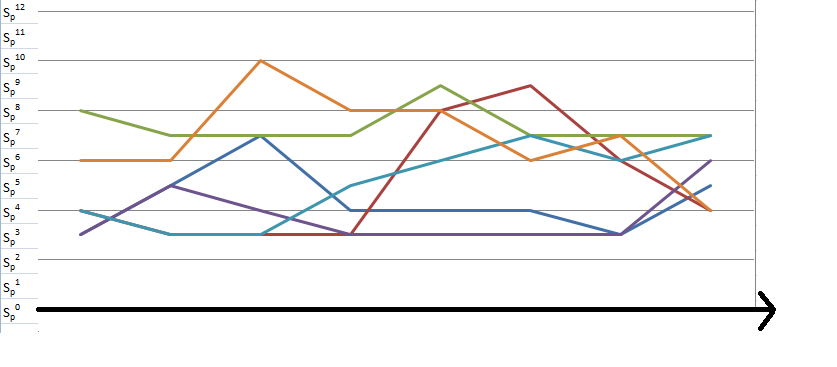
\includegraphics[width=150mm, keepaspectratio]{figures/trajectory1.png}
	\caption{\label{fig:trajectory1}An example trajectories for P}
\end{figure}

For example we want to test that certain states ($S_{P}^{0}$, $S_{P}^{1}$, $S_{P}^{2}$, $S_{P}^{11}$, $S_{P}^{12}$) can be reached at any execution. We have to check every possible trajectory and if none of trajectories contains them than we can say they are unreachable otherwise we can find a counter example. Usually we define error states, what we do not want to reach. We need to prove that none of the trajectories contains error states. 

\begin{figure} [!ht]
	\centering
	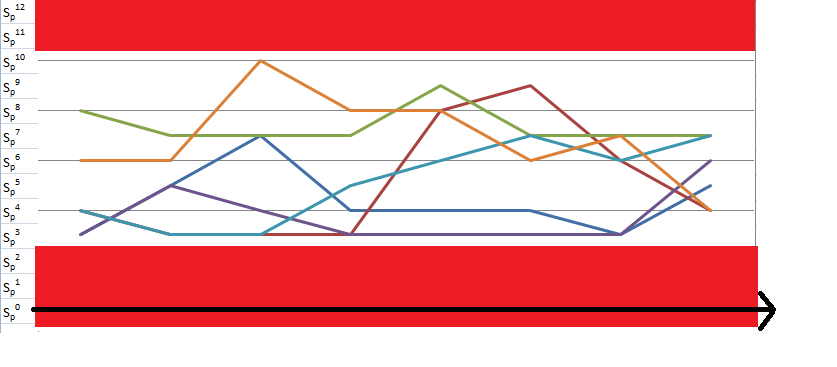
\includegraphics[width=150mm, keepaspectratio]{figures/trajectory2.png}
	\caption{\label{fig:trajectory2}Red shows the error states}
\end{figure}

\begin{figure} [!ht]
	\centering
	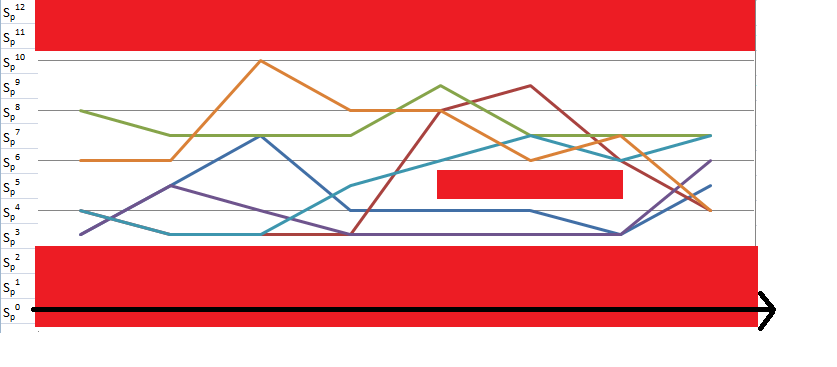
\includegraphics[width=150mm, keepaspectratio]{figures/trajectory3.png}
	\caption{\label{fig:trajectory3}Error state can be time dependent}
\end{figure}

Finding a \hyperref[fig:trajectory4]{counter example} is easier than proving that there is no trajectory which contains error states. 

\begin{figure} [!ht]
	\centering
	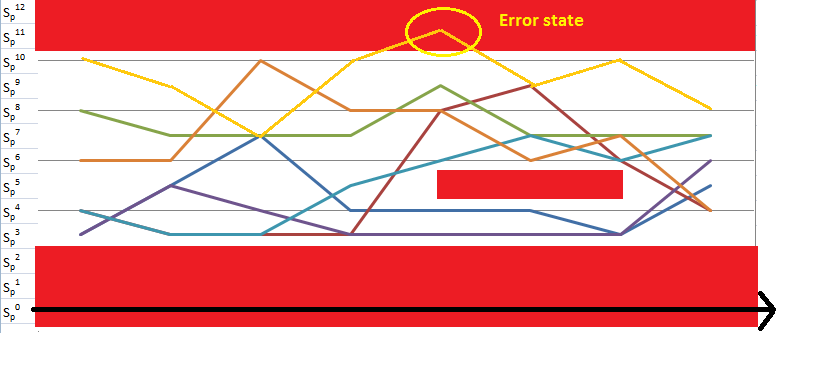
\includegraphics[width=150mm, keepaspectratio]{figures/trajectory4.png}
	\caption{\label{fig:trajectory4}A counter example}
\end{figure}


The problem is that not only there could be many (even infinite) possible trajectories, but some of these can also be infinite. So iterating through all of them is impossible within reasonable time.


%----------------------------------------------------------------------------
\section{Abstraction}
\label{sec:abstraction}
%---------------------------------------------------------------------------- 

The goal of the abstraction is to make it possible to compute in reasonable time that a certain state is reachable or not. Consider what makes it impossible.

(1) P[S] can be infinite
(2) $T_{P}$ can be infinite
(3) there can be infinite number of $T_{P}$-s
  
Abstraction is possible on the states that represents the program. S' is the abstracted state:

$S_{P}^{'1}=S_{P}^{1} \cup S_{P}^{2} \cup S_{P}^{3}$

$S_{P}^{'2}=S_{P}^{4}$

than

$P[S]={S_{P}^{1}, S_{P}^{2}, S_{P}^{3}, S_{P}^{4}}$

$P[S']={S{P}^{'1}, S_{P}^{'2}}$

$T={S_{P}^{1}, S_{P}^{4}, S_{P}^{3}}$

$T'={S_{P}^{'1}, S_{P}^{'2}, S_{P}^{'1}}$

if $S_{P}^{i}$ is error state and $S_{P}^{i} \in S_{P}^{'i}$ than $S_{P}^{'i}$ is error state

Even if the program had infinite states it can now be narrowed to a finite number. For example we define a default S' which contains every state that is not in the other (already abstracted) states. So problem (1) is solved.
 
Fixpoint: Let $T_{P}={S_{P}^{1}, S_{P}^{3}, S_{P}^{5}, ..., *}$ be an infinite trajectory. A fixpoint is the first point, where there are no new states in the trajectory
Formally: (FP=Fixpoint) $min(FP)$ where $T_{P}^{before FP}=$trajectory before Fixpoint, $T_{P}^{after FP}=$trajectory after Fixpoint than $T_{P}^{after FP}[S] \subseteq T_{P}^{before FP}[S]$

We can abstract the infinite trajectory by its sub trajectory before the fix point
Formally  $T_{P}={S_{P}^{1}, S_{P}^{3}, S_{P}^{5}, ..., *}$ and $T'_{P}= T_{P}^{before FP}$ 

By this we do not lose any states that we reached, and if $P[S]$ is finite than $T'_{P}$ will be finite as well. So problem (2) is solved.

Problem (3) is solved, because there are maximum $(longest trajectory)^{|P(S')|}$ trajectories.

Figure \hyperref[fig:trajectory7]{2.5} shows a reachability check where the states abstraction: $P[S']=\{S_{P}^{'error}, S_{P}^{'error!}\}$ where $S_{P}^{'error}=\{S_{P}^{0}$, $S_{P}^{1}$, $S_{P}^{2}$, $S_{P}^{11}$, $S_{P}^{12}\}$ and $S_{P}^{'\not error}=\{S_{P}^{3-10}\}$

 \begin{figure} [!ht]
 	\centering
 	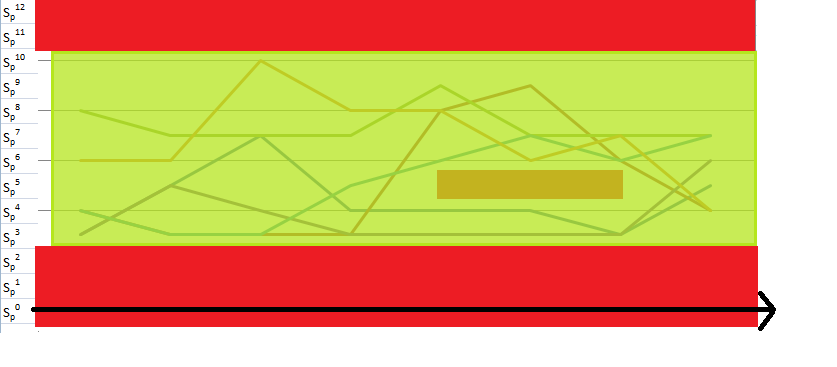
\includegraphics[width=150mm, keepaspectratio]{figures/trajectory7.png}
 	\caption{\label{fig:trajectory7}Reachability check with abstraction}
 \end{figure}


%----------------------------------------------------------------------------
\section{Partition}
\label{sec:partition}
%---------------------------------------------------------------------------- 

Figure \hyperref[fig:trajectory7]{2.5} shows that with the abstraction we proved that $S_{P}^{0}$, $S_{P}^{1}$, $S_{P}^{2}$, $S_{P}^{11}$, $S_{P}^{12}$ states are unreachable, however it can not prove that $S_{P}^{8}$ will not be reached at an erroneous
time. This happens, because during abstraction we lose information.

\begin{theorem}
	It is more important to detect that an error state is reachable than to prove that it is not. This means that, if we say a certain error state is reachable even though it is not then it is tolerable, however if we say it is not reachable even though it is, then it is not tolerable. 	
\end{theorem}
{proof: } The effects of false positive (we said it is reachable, but it was not) will not have any harm, as the programmer can detect that and then he will not take the result into account. However the false negative (we said it is unreachable, but it was) can have severe damage since, the programmer can assume that there is no fault, and if the error occurs especially in safety-critical systems it has serious effects.

One solution for this problem is partition.

 \begin{figure} [!ht]
	\centering
	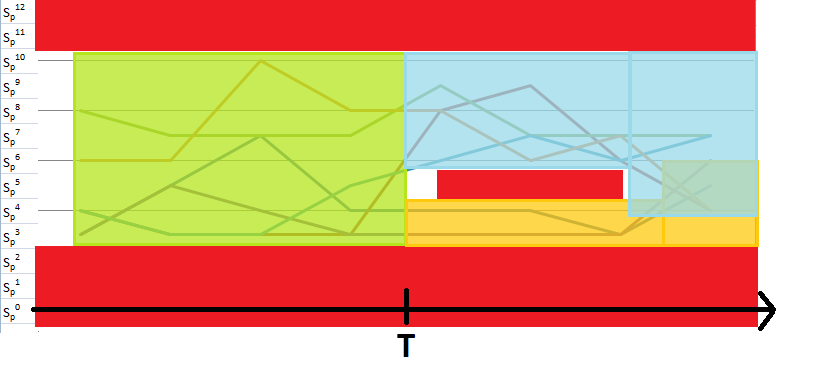
\includegraphics[width=150mm, keepaspectratio]{figures/trajectory8.png}
	\caption{\label{fig:trajectory8}Partition example}
\end{figure}

 In figure \hyperref[fig:trajectory7]{2.6} We start with the same abstraction as in \hyperref[fig:trajectory7]{2.5}, but at T we use partitioning. $P[S']=\{S_{P}^{'error}, S_{P}^{'1} , S_{P}^{'2}\}$ where $S_{P}^{'1}=\{S_{P}^{3}$, $S_{P}^{4}\}$ and $S_{P}^{'2}=\{S_{P}^{6}$, $S_{P}^{7}$, $S_{P}^{8}$, $S_{P}^{9}$, $S_{P}^{10}\}$

%----------------------------------------------------------------------------
\section{Widening}
\label{sec:widening}
%---------------------------------------------------------------------------- 

\begin{definition}{Bound}
	A Bound is a specified whole number or Infinite (can be positive or negative) $Bound \in \mathbb{Z} \lor Bound \in \{ +\infty, -\infty \}$
\end{definition}

\begin{definition}{max($Bound1$, $Bound2$)=}
	
	if $Bound1 == +\infty \lor Bound2 == +\infty$ then $+\infty$
	
	else if $Bound1 == -\infty \lor Bound1<Bound2$ then $Bound2$
	
	else $Bound1$	
\end{definition}

\begin{definition}{min($Bound1$, $Bound2$)=}
	
	if $Bound1 == -\infty \lor Bound2 == -\infty$ then $-\infty$
	
	else if $Bound1 == +\infty \lor Bound1>Bound2$ then $Bound2$
	
	else $Bound1$	
\end{definition}

\begin{definition}{$Bound+K \in \mathbb{Z}$)=}
	
	if $Bound == +\infty \lor Bound == -\infty$ then $Bound1$
	
	else ($Bound \in \mathbb{Z}$) then $Bound+K$
\end{definition}

\begin{definition}{$|Bound|$=}
	
	if min($Bound$, $0$) $==0$ then $Bound$
	
	else $Bound*(-1)$
\end{definition}

Or

\begin{definition}{$|Bound|$=}
	
	if $Bound \in  \mathbb{Z}$ then $|Bound|$ is the regular $absolute function$ in $\mathbb{Z}$
	
	else $|Bound| = +\infty$
\end{definition}

\begin{definition}{Interval}
	An interval is specified with two Bounds: the lower Bound($LB$) and the higher Bound($HB$).
	
	ex.: $(2;+\infty)$, $(3;1)$
\end{definition}

\begin{definition}{Interval is valid}
	
	if min($LB$, $HB$) == $LB \neq +\infty \land$ max($LB$, $HB$) == $HB  \neq -\infty$
	
	Note: empty interval ($Ei$) $\equiv$ invalid interval
	
	Note2: intervals $(+\infty, +\infty)$, $(-\infty, -\infty)$ are also empty intervals 
	
	ex.: $(2;+\infty)$ and $(0;0)$ is valid, but $(3;1)$ is not valid $\equiv$ invalid
\end{definition}

\begin{definition}{Initial interval ($Ii$)=}
	
	An Interval where
	
	$LB$=$-\infty$
	
	$RB$=$+\infty$
	
	Initial interval $\equiv \Omega$ where $\Omega$ is the Full set of possible values
	
	($-\infty$,$+\infty$)
\end{definition}

\begin{definition}{inside $k \in Interval$}
	
	let $k$ be $\in \mathbb{Z}$ and interval $Int$ be ($k$, $k$). then if $Int \cup Interval$ == $Int$ we say $k$ is inside $Interval$
	
	ex.: $7 \in (2,7)$
\end{definition}



%----------------------------------------------------------------------------
\chapter{Background}
\label{sec:cfa}
%----------------------------------------------------------------------------


%----------------------------------------------------------------------------
\section{program representation}
%---------------------------------------------------------------------------- 

A program most commonly is represented by a source code. Example: an average counter function in c

\begin{lstlisting}[language=C,breaklines=true]
int average(int a, int b){
int avg;
avg=(a+b)/2;
return avg;
}
\end{lstlisting}

There are many different type of code languages, making a static analyzer for all, would be hard and unnecessarily time-consuming. 

%----------------------------------------------------------------------------
\section{\cfa (CFA)}
\label{sec:cfaleiras}
%---------------------------------------------------------------------------- 
CFA can describe the programs as graphs, where edges are annotated with program statements. The Theta framework \hyperref[sec:ref]{[4]} provides a representation of a CFA formalism.

A CFA is a directed graph with
 
\begin{itemize}
	\item variables,
	\item locations, with dedicated initial, final and error locations,
	\item edges between locations, labeled with statements over the variables.
\end{itemize}

\begin{enumerate}
	\item Assume: check if a condition is true for the variables
	\item Assign: assign a concrete value to a variable
	\item Havoc: assign a random value to a 
	\item Skip: no action
\end{enumerate}

\label{fig:simpleC}This simple C code translates to 5 location:
\begin{lstlisting}[language=C,breaklines=true]
//Loc1
int a=1;
//Loc2
if(a!=1){
	//errorLOC
}
else {
//Loc3
	printf("%d", a);
}
//Loc4
\end{lstlisting}

The edges are the program statements. For example from Loc1 to Loc2 an assign statement which set a variable to 1, and from Loc2 to Loc3 is an assume statement (!(a!=1)).

Analysis is usually made for reachability of the error state.


%----------------------------------------------------------------------------
\section{Motivation}
\label{sec:motibation}
%----------------------------------------------------------------------------

Why do we need abstraction? 

%----------------------------------------------------------------------------
\section{Abstraction in general}
\label{sec:general}
%----------------------------------------------------------------------------

%----------------------------------------------------------------------------
\section{Abstraction analysis algorithm for CFA}
\label{sec:cfaalgorithm}
%---------------------------------------------------------------------------- 

\begin{figure} [!ht]
	\centering
	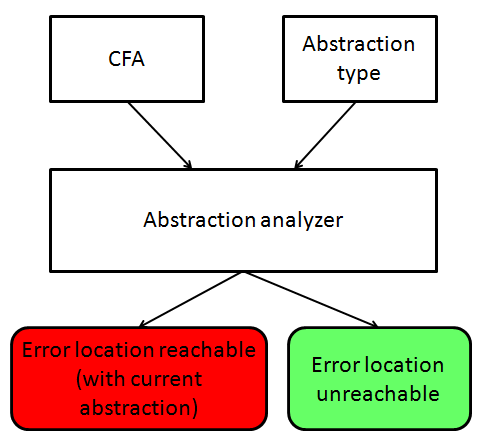
\includegraphics[width=100mm, keepaspectratio]{figures/abstractanalyzer.png}
	\caption{\label{fig:absanalyzer} Abstraction analysis model}
\end{figure}

The CFA provides only one error state. This is not a problem since if there is more, then a simple abstraction can make one error state that contains all.

$\forall i$ $S_{P}^{i} \in $ Error states $S_{P}^{'error}=\cup S_{P}^{i}$

Label: representation of the Program. (in section \hyperref[sec:saai]{SAAI} these were the states of the program  $S_{P}^{i}$). Usually it will be a representation of the CFA's variables.

Every abstraction type need to have its own Label type. For example in case of sign abstraction a label type would be a (-), (+) or (-+) assigned to every variable (meaning: it can only be minus, it can only be positive, it can be both).

The possible trajectories are represented in the CFA by iterations of the CFA graph. So the problem of reaching the error states, in CFA means that there is no valid path from the initial location to the error location. Valid means that every edge in the path is a possible step.

For example a possible trajectory in \hyperref[fig:simpleC]{the code from the previous section} is Loc1, Loc2, Loc3, Loc4 (this is the only possible trajectory since Loc2 -> errorLoc edge is an impossible step (a is 1)).

The validation test on an edge is only possible if we put labels to the locations and from the label it is possible to decide that an edge is valid or not. Note: the edge can only be invalid if it has an assume statement
For example if we use sign abstraction and on LocationA we have a label that $var=(+)$ than we can decide wether edge LocationA -> LocationB is valid or not. For example $var>0$ is valid, but $var<0$ is not.

Apply the statement:
If an edge is valid, than we put a new label to the target location (the target of the edge) according to the statement on the edge.
It has two different cases; if the target does not have a label, that means we have reached it for the first time. In this case from the source's label and the edge's statement, we need to be able, to decide the targets label. This is actually depending on the partition tactic (\hyperref[sec:partition]{see Partition in previous chapter}).
If the target already has a label we need to take it into account. This is depending on the widening tactic (\hyperref[sec:widening]{see Widening in previous chapter}).  

Discovered locations:
All the locations that have been reached, and therefore have a label.

Discovered mapping:
Every discovered location mapped with its label. When we apply a statement we modify the Discovered mapping (change the label for one location or add a completely new location).

Modifying edge:
All the outgoing edges from those locations whose label have been modified from the previous Discovered mapping

Fixpoint:
The point where the Discovered mapping can not be changed anymore. So there is no more modifying edges. Note: this is equivalent to: the previous Discovered mapping is the same as the current one (if we applied all the modifying edges from the previous discovered mapping).

Initial step: we put a label on the initial location (it is given in the CFA). Therefore every label type should have an initial label. It represents the program state, where we do not know anything, for example in sign abstraction every variable should be assigned to (+-), since both (+) and (-) can be true.

Iteration:
Let there be a set of discovered locations $D(L)$, and a discovered mapping $M(Loc, Label)^{n}$ and the error location is $ELOC$.
If $ELOC \in D(L)$ we can stop the iteration we reached the error location.
Otherwise If $M(Loc, Label)^{n-1} == M(Loc, Label)^{n}$ we can stop there are no more modifying edges we reached a fixpoint therefore the error location is not reachable.
If $M(Loc, Label)^{n-1} != M(Loc, Label)^{n}$ than we get all the modifying edges from $M(Loc, Label)$ and apply all of the statements in the modifying edges.
If one location is modified by more than one statement we add these labels together, for example in sign abstraction $var=(-)$ and $var=(+)$ are the two modifying statements, then we put $var=(-+)$. So labels should also support this operation. 

If a location is reached and labeled, than its new label can only be less specific.
For example in sign abstraction LocA has a $var=(+-)$ label than if there is a statement which assigns $var=(+)$ it can not narrow down LocA's label as in LocA (-) is already possible (in at least one trajectory).

Partitioning and widening can differ according to what type of abstraction are we using.

\begin{figure} [!ht]
	\centering
	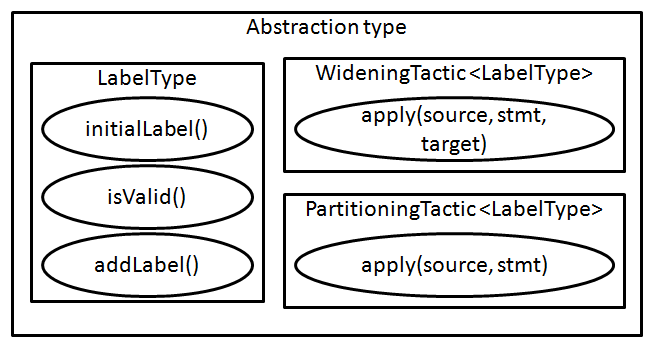
\includegraphics[width=150mm, keepaspectratio]{figures/abstractiontype.png}
	\caption{\label{fig:abstype} The structure of an Abstraction type}
\end{figure}










%----------------------------------------------------------------------------
\chapter{Abstract Interpretation with Intervals}
\label{sec:intervalabstraction}
%----------------------------------------------------------------------------

%----------------------------------------------------------------------------
\section{Library}
%---------------------------------------------------------------------------- 

\begin{definition}{Bound}
	A Bound is a specified whole number or Infinite (can be positive or negative) $Bound \in \mathbb{Z} \lor Bound \in \{ +\infty, -\infty \}$
\end{definition}

\begin{definition}{max($Bound1$, $Bound2$)=}

	if $Bound1 == +\infty \lor Bound2 == +\infty$ then $+\infty$
	
	else if $Bound1 == -\infty \lor Bound1<Bound2$ then $Bound2$
	
	else $Bound1$	
\end{definition}

\begin{definition}{min($Bound1$, $Bound2$)=}

if $Bound1 == -\infty \lor Bound2 == -\infty$ then $-\infty$

else if $Bound1 == +\infty \lor Bound1>Bound2$ then $Bound2$

else $Bound1$	
\end{definition}

\begin{definition}{$Bound+K \in \mathbb{Z}$)=}
	
	if $Bound == +\infty \lor Bound == -\infty$ then $Bound1$
	
	else ($Bound \in \mathbb{Z}$) then $Bound+K$
\end{definition}

\begin{definition}{$|Bound|$=}
	
	if min($Bound$, $0$) $==0$ then $Bound$
	
	else $Bound*(-1)$
\end{definition}
	
	Or
	
\begin{definition}{$|Bound|$=}
	
	if $Bound \in  \mathbb{Z}$ then $|Bound|$ is the regular $absolute function$ in $\mathbb{Z}$
	
	else $|Bound| = +\infty$
\end{definition}

\begin{definition}{Interval}
	An interval is specified with two Bounds: the lower Bound($LB$) and the higher Bound($HB$).
	
	ex.: $(2;+\infty)$, $(3;1)$
\end{definition}

\begin{definition}{Interval is valid}
	
	if min($LB$, $HB$) == $LB \neq +\infty \land$ max($LB$, $HB$) == $HB  \neq -\infty$
	
	Note: empty interval ($Ei$) $\equiv$ invalid interval
	
	Note2: intervals $(+\infty, +\infty)$, $(-\infty, -\infty)$ are also empty intervals 
	
	ex.: $(2;+\infty)$ and $(0;0)$ is valid, but $(3;1)$ is not valid $\equiv$ invalid
\end{definition}

\begin{definition}{section of two intervals $Interval1 \cap Interval1$=}
	
	if $Interval1, Interval2$ is valid then 
	
	$LB$=max($Interval1.LB$, $Interval2.LB$)
	
	$RB$=min($Interval1.HB$, $Interval2.HB$)
	
	else $Ei$
	
	ex.: $(2,8)\cap(1,3)=(2,3)$, $(2,8)\cap Ei=Ei$
\end{definition}

\begin{definition}{union of two intervals $Interval1 \cup Interval1$=}
	
	if $Interval1, Interval2$ is valid then 
	
	$LB$=min($Interval1.LB$, $Interval2.LB$)
	
	$RB$=max($Interval1.HB$, $Interval2.HB$)
	
	else if $Interval1$ is valid then $Interval1$
	
	else if$ Interval2$ is valid then $Interval2$
	
	else $Ei$
	  
	ex.: $(2,8)\cup(1,3)=(1,8)$, $(2,8)\cup Ei=(2,8)$
\end{definition}

\begin{definition}{subtraction of two intervals (no partition) $Interval1 \setminus Interval2$=}

if $Interval1$, $Interval2$ is valid then 

if min($Interval1.LB$, $Interval2.LB$)==$Interval2.LB$ $\land$ max($Interval1.HB$, $Interval2.HB$)==$Interval2.HB$ then 
$Ei$

else

$Interval2.LB$=$Interval2.LB-1$

$Interval2.HB$=$Interval2.HB+1$

if min($Interval1.LB$, $Interval2.LB$)==$Interval1.LB$ $\land$ max($Interval1.HB$, $Interval2.HB$)==$Interval1.HB \land Interval2.LB \neq -\infty \land Interval2.HB \neq +\infty$ then $Interval1$

else if min($Interval1.LB$, $Interval2.LB$)==$Interval1.LB$ $\land$ max($Interval1.HB$, $Interval2.HB$)==$Interval1.HB \land Interval2.LB == -\infty \land Interval2.HB \neq +\infty$ then 

$LB$=$Interval2.HB$

$HB$=$Interval1.HB$

else if min($Interval1.LB$, $Interval2.LB$)==$Interval1.LB$ $\land$ max($Interval1.HB$, $Interval2.HB$)==$Interval1.HB \land Interval2.LB \neq -\infty \land Interval2.HB == +\infty$ then 

$LB$=$Interval1.LB$

$HB$=$Interval2.LB$

else if min($Interval1.LB$, $Interval2.HB$)==$Interval2.HB$ $\lor$ max($Interval1.HB$, $Interval2.LB$)==$Interval2.LB$ then $Interval1$

else if min($Interval1.LB$, $Interval2.LB$)==$Interval2.LB$ $\land$ max($Interval1.HB$, $Interval2.HB$)==$Interval1.HB$ then

$LB$=$Interval2.HB$

$HB$=$Interval1.HB$

else if min($Interval1.LB$, $Interval2.LB$)==$Interval1.LB$ $\land$ max($Interval1.HB$, $Interval2.HB$)==$Interval2.HB$ then

$LB$=$Interval1.LB$

$HB$=$Interval2.LB$

if $Interval2$ is invalid then $Interval1$

else $Ei$

for visual representation (\hyperref[fig:aminusb]{see figure 4.1} )

ex.: $(4,6)\setminus(1,8)=Ei$, $(2,8)\setminus(4,6)=(2,8)$, $(5,8)\setminus(1,4)=(5,8)$, $(1,4)\setminus(5,8)=(1,4)$, $(1,6)\setminus(3,8)=(1,2)$, $(3,8)\setminus(1,6)=(7,8)$, $Ei\setminus(1,6)=Ei$
\end{definition}

\begin{figure} [!ht]
	\centering
	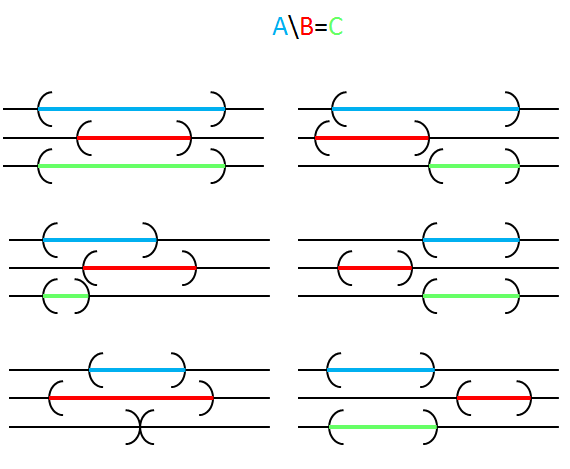
\includegraphics[width=150mm, keepaspectratio]{figures/aminusb.png}
	\caption{\label{fig:aminusb} Interval $A$ $\setminus$ Interval $B$ possible outcomes}
\end{figure}

\begin{definition}{Initial interval ($Ii$)=}
	
	An Interval where
	
	$LB$=$-\infty$
	
	$RB$=$+\infty$
	
	Initial interval $\equiv \Omega$ where $\Omega$ is the Full set of possible values
	
	($-\infty$,$+\infty$)
\end{definition}


\begin{definition}{complementer of an interval$ \overline{Interval}$=}
	
	$Ii \setminus Interval$
	
	ex.: $\overline{(2,8)}=(-\infty,+\infty)$ ($Ii$), $\overline{(-\infty,8)}=(9,+\infty)$, $\overline{Ei}=(Ii)$
\end{definition}

\begin{definition}{inside $k \in Interval$}
	
	let $k$ be $\in \mathbb{Z}$ and interval $Int$ be ($k$, $k$). then if $Int \cup Interval$ == $Int$ we say $k$ is inside $Interval$
	
	ex.: $7 \in (2,7)$
\end{definition}




%----------------------------------------------------------------------------
\section{Interval representation}
%---------------------------------------------------------------------------- 
\begin{definition}
Interval representation is a label for interval abstraction. It maps an interval to every variable. The possible values are inside the given intervals for every variable.
\end{definition}

\begin{theorem}	
	Let there be an Interval representation, where we map an Initial interval ($Ii$) to every variable. This interval representation is a good initial label for the abstraction analysis.
\end{theorem}

\begin{definition}
	Let there be an Interval representation. If every variable is mapped with a valid interval then we say the Interval Representation is .
\end{definition}

\begin{theorem}	
	Let there be two Interval representation $Ier1$ and $Ier2$ to the same program so it has the same variables. To every variable we map \[Ier1.IntervalforVar \cup Ier2.IntervalforVar\]This is a good $addLabel()$ function for the abstract analysis.
\end{theorem}
	
	{proof:} Let us say that this is not a good $addLabel()$ function. That means that exists a variable value that is allowed by one of the Interval representation, but is not allowed in \[Ier1.IntervalforVar \cup Ier2.IntervalforVar\] however this contradicts with the definition of the union of two intervals. So this should be a good $addLabel()$ function.	

%---------------------------------------------------------------------------
\section{No Partitioning Tactic<Interval representation>}
%---------------------------------------------------------------------------- 

\begin{definition}
	No Partitioning Tactic<Interval representation> is a Partitioning tactic for abstract analysis using Interval Representation as abstraction label.
\end{definition}

Every Partitioning Tactic should define how to set the target's label from a source's label and an edge's statement.

\begin{definition}
	Let there be an Interval $Interval$ and a statement $stmt$. Then we can apply $stmt$ to $Interval$ and it results in a new Interval. ($Interval.apply(stmt)$)
\end{definition}

Let there be a source's Interval representation $IerS$ and a statement $stmt$. No Partitioning Tactic<Interval representation> maps every variable to $IesS.IntervalforVar.apply(stmt)$.

\begin{theorem}
	Let there be an Interval $Interval$ for variable $var$ and a statement $stmt$. If $stmt$ has no effect on $var$ then
	$Interval.apply(stmt)=Interval$ 
\end{theorem}

{proof: } every possible values in the source location will be possible in the target location, and if a value is not allowed in the source location it will not be allowed in the target location since nothing has changed regarding the variable

\begin{theorem}
	Let there be an Interval $Interval$ for variable $var$ and a Skip statement $skipstmt$.It has no effect on the variable.
\end{theorem}
{proof: }it is directly comes from the definition of Skip statement. \hyperref[sec:cfaleiras]{see CFA section}

\begin{theorem}
	Let there be an Interval $Interval$ for variable $var$ and a Havoc statement $havstmt$. If $havstmt$ sets $var$ then
	$Interval.apply(havstmt)=Ii$. Otherwise it has no effect on the variable.
\end{theorem}

{proof: } if the statement sets the variable it means it can have any values. So we must represent the variable with $\Omega \equiv Ii$. Setting another variable does not have any effect on the current variable.


%---------------------------------------------------------------------------
\section{Applying Assign statement}
%---------------------------------------------------------------------------- 


\begin{definition}
	Let there be an Assign statement $assignstmt$. Then the interval that represents all the possible values allowed by the assignment is $assignstmt.transform$.
\end{definition}

\begin{theorem}
	Let there be an Interval $Interval$ for variable $var$ and an Assign statement $assignstmt$. If $assignstmt$ sets $var$ then
	$Interval.apply(assignstmt)=assignstmt.transform$. Otherwise it has no effect on the variable.
\end{theorem}
{proof: } if the statement sets the variable it means it will have the value given by the assignment. So we must represent the variable with the Interval that represents any values allowed by the assignment which is $assignstmt.transform$. Setting another variable does not have any effect on the current variable.

An assignment is made of Expressions. Using the Theta Framework \hyperref[sec:ref]{[4]} and considering only the integer type expressions the possibilities are as follows
\begin{itemize}
	\item Divide ($IntDivExpr$)
	\item Add ($IntAddExpr$)
	\item Subtract ($IntSubExpr$)
	\item Reference ($refExpr$) for variables.
	\item Literal ($IntLitExpr$) for literal expressions like 4 or 0
\end{itemize}

\begin{theorem}
	Let $k$ be a literal expression then the Interval that represents the possible values is $(k, k)$
\end{theorem}
{proof: } The only possible value is $k$

\begin{theorem}
	Let $Interval$ be a representation for possible values for variable $var$. Then a reference expression referencing $var$ can be represented with $interval$.
\end{theorem}
{proof: } The possible values are the same as it was before.

\begin{theorem}
	Let $EXpr1$, $EXpr2$, ... ,$EXprn$ be expressions represented by $Interval1$, $Interval2$, ..., $Intervaln$. then the Interval representation for $Add(EXpr1, EXpr2, ... ,EXprn)$ is
	
	if $Interval1.LB, Interval2.Lb, ... ,Intervaln.LB == -\infty$ then $result.LB=-\infty$
	else  $result.LB=\sum{Intervali.LB}$
	
	if $Interval1.HB, Interval2.Hb, ... ,Intervaln.HB == +\infty$ then $result.LB=+\infty$
	else  $result.LB=\sum{Intervali.HB}$
\end{theorem}
{proof: } the highest possible value is that every expression has the highest value. If all of them is finite then the biggest value is the sum of these, otherwise it is infinite. The lowest possible value is similar.

\begin{theorem}
	Let $EXpr1$, $EXpr2$ be expressions represented by $Interval1$, $Interval2$. Then the Interval representation for $Sub(EXpr1, EXpr2)$ is $result$ where:
	
	$result.LB=-\infty$ //initially
	
	$result.HB=+\infty$ //initially
	
	if $Interval1.HB \neq +\infty \land Interval2.LB \neq -\infty$ then 
	
	$result.HB=Interval1.HB-Interval2.LB$ ($Interval2.LB, Interval1.HB \in \mathbb{Z}$)
	
	if $Interval1.LB \neq -\infty \land Interval2.HB \neq \infty$ then 
	
	$result.LB=Interval1.LB-Interval2.HB$ ($Interval1.LB, Interval2.HB \in \mathbb{Z}$)
	
\end{theorem}
{proof: } Starting as every values will be possible. We can decide the maximum value by subtracting the lowest possible value from the highest possible value. Let the values be $a$ and $b$ where we want to calculate $a-b$ and $a, b \in \mathbb{Z}$ then $a-b>c-b$ if $a>c$ and $a-b>a-c$ if $b<c$. The lowest possible value is similar.


\begin{theorem}
	If we put more possible values to the assignment result we do not lose any possible values	
\end{theorem}
{proof: }If a value is possible and we put other possibilities as well, it is trivial that the original value will still be possible.

 Of course we might have some values that is incorrect, however as said in \hyperref[sec:partition]{the SAAI chapter} it is tolerable to say that something is reachable even though it is not. 

\begin{theorem}
	Let $EXpr1$, $EXpr2$ be expressions represented by $Interval1$, $Interval2$. Then the Interval representation for $Div(EXpr1, EXpr2)$ is 
	
	if $Interval1.LB \neq -\infty \land Interval1.HB \neq +\infty$ then 
	
		$A = $max( $|Interval1.LB|$ , $|Interval1.HB|$ )
	
		if($0$ is inside $Interval2$) then $B = 1$		
	
		else $B = $min( $|Interval1.LB|$ , $|Interval1.HB|$ )		
		
		$Div(EXpr1, EXpr2).HB = A/B$
		
		$Div(EXpr1, EXpr2).LB = -A/B$
		
	else
	
		$Div(EXpr1, EXpr2) = Ii$
	
\end{theorem}
{proof: } We simplify the problem by omitting the signs of the Bounds. This helps in the problem of sign changes (like (+)/(-)=(-)).  We do not lose any possible values since we search for the highest possible absolute value and the interval will be $(-highest, highest)$. Now if $Interval1$ biggest absolute value is infinite then the result will be infinite as well. ($\infty / a = \infty)$ If it is finite then let as consider $a$ and $b$ where $a, b \in \mathbb{Z}^{+}$.Then $a/b > c/b$ if $a>c$ and $a/b > a/c$ if $b<c$. So in $Interval1$ we search for the highest possible absolute value in $Interval2$ for the lowest possible value. If $interval2$ is just positive or negative then the the lowest absolute value is on the bound, otherwise it contains 0. Zero division is not allowed, however our abstraction sometimes put 0 into the possibilities even though it is not possible. (For instance after division we always put 0 in the possible values, however it is only possible if the dividend is zero) So if we omit the 0 value then the next smallest absolute value is 1.

\begin{theorem}
	Let $EXpr1$, $EXpr2$, ... ,$EXprn$ be expressions represented by $Interval1$, $Interval2$, ..., $Intervaln$. then the Interval representation for $Mul(EXpr1, EXpr2, ... ,EXprn)$ is
	
	if $Interval1.LB, Interval2.Lb, ... ,Intervaln.LB == -\infty \lor +\infty$ then 
	
	$Mul(EXpr1, EXpr2, ... ,EXprn)=Ii$
	
	else
	
	$Mul(EXpr1, EXpr2, ... ,EXprn)= \Pi $max($|Intervali.LB|$, $|Intervali.HB|$)
\end{theorem}
{proof: } We simplify the problem by omitting the signs of the Bounds. This helps in the problem of sign changes (like (+)/(-)=(-)).  We do not lose any possible values, because we search for the highest possible absolute value and the interval will be $(-highest, highest)$, so we only add more values. The biggest possible absolute value is when every multiplier has its highest possible value. If any multiplier is $\infty$ then the result is of course $Ii$


%---------------------------------------------------------------------------
\section{Applying Assume statement}
%---------------------------------------------------------------------------- 

\begin{definition}
	Let there be an Assume statement $assumestmt$ and a variable $var$. Then the interval that represents the values where the assumption is feasible for $var$ is $assumestmt.transform$.
\end{definition}

\begin{theorem}
	Let there be an Interval $Interval$ for variable $var$ and an Assume statement $assumestmt$. If $assumestmt$ has a condition to $var$ then
	$Interval.apply(assumestmt)=assumestmt.transform$. Otherwise it has no effect on the variable.
\end{theorem}
{proof: } If the statement has condition for the variable it means it will have the value allowed by the assumption. So we must represent the variable with the Interval that represents any possible values in the assumption which is $assumestmt.transform$.

\begin{theorem}
	An Assume statement can only narrow down the possible values.
\end{theorem} 
{proof: } If a value is not allowed in the source location, then it will not be possible in the target location since we, do not change the variable

The consequence of this theorem is this next theorem:
\begin{theorem}
	Let there be an Interval $Interval$ for variable $var$ and an Assume statement $assumestmt$. We do not lose any possible values if $Interval.apply(assumestmt)=Interval$
\end{theorem} 

\begin{definition}
	A $condition$ is an interval, which represents the possible values for a variable (can be calculated from any Expression used in the assignment).
\end{definition}

\begin{definition}
	We say an assumption is trivial for a variable $var$ if it is in a form of: $var \{==, \neq, \geq, >, \leq, < \} condition$ where $condition$ is an interval (it can be calculated from any Expression used in the assignment, but shall not depend on $var$)
\end{definition}

\begin{definition}
	Let variable $var$ be represented by $interval$. An incorrect value is inside $interval$,  but $var$ is not allowed to have this value.
\end{definition}

\begin{definition}
	An incorrect condition is a $condition$, which is an interval that may have incorrect values.
\end{definition}

\begin{theorem}
	A trivial condition is then and only then incorrect, if the $condition$ is calculated using reference, multiply or divide expression
\end{theorem} 
{proof: } then:

 Reference expression can be represented by an interval for a variable, which allows incorrect values.
 
 Multiply, and divide expression both uses over exaggeration for the possible values.
 
 only then: all the other possible assignments allow only the possible values. 

\begin{definition}
	We say an Assume statement is applicable for a variable if the statement consists of $AND$, $OR$ or $NOT$ functions of a trivial assumption for the variable. It is not applicable though if the Assume statement has incorrect condition.
\end{definition}

Let there be an Interval $Interval$ for variable $var$ and an Assume statement $assumestmt$. if $assumestmt$ is not applicable $assumestmt.transform = Interval$. We can do this because of Theorem 17


\begin{theorem}
	Let there be a trivial assumption for variable $var$ represented by $IntervalVar$ where the assumption's $condition$ is correct and represented by $IntervalCondition$
	
	then
	
	$var \geq condition=($max($IntervalCondition.LB$, $IntervalVar.LB$),$IntervalVar.HB)$
	
	ex. $(3, 7) \geq (1,5) = (3,7)$, $(3, 7) \geq (5,5) = (5,7)$
	
	$var \leq condition=(IntervalVar.LB$, min($IntervalCondition.HB$, $IntervalVar.HB))$
	
	ex. $(3, 7) \leq (1,5) = (3,5)$, $(3, 7) \leq (1,1) = (3,1) \equiv Ei$
	
	$var > condition=($max($IntervalCondition.LB+1$, $IntervalVar.LB$),$IntervalVar.HB)$
	
	ex. $(3, 7) > (3,5) = (4,7)$, $(3, 7) > (2,5) = (3,7)$
	
	$var < condition=(IntervalVar.LB$, min($IntervalCondition.HB-1$, $IntervalVar.HB))$
	
	ex. $(3, 7) < (1,5) = (3,4)$, $(3, 7) < (3,3) = (3,2) \equiv Ei$
	
	$var \neq condition=var \setminus condition$
	
	ex.  $(3, 7) \neq (1,5) = (6,7)$, $(6, 7) \neq (1,5) = (6,7)$
	
	$var == condition = var \cup condition$
	
	ex.  $(3, 7) == (1,5) = (1,5)$, $(6, 7) == (1,5) = Ei$
	
	Note: $\neq$ is the only one that can make incorrect possible values. For example $(3, 7) \neq (4,5) = (3,7)$ however $4$ and $5$ are incorrect. Still we only allow more possibilities.
	
\end{theorem}
{proof: } $<, >$: Let $var > condition$ be $(a, b)>(c, d)$ and valid then $var > condition=(max(a, c+1), b)$ 

if $a>c+1$ then

 $\forall i \in (a, b), \exists j \in (c, d)$ where $ i>j$ so it is true and 
 
 $\forall i \notin (a, +\infty), \nexists j \in (a, b)$ where $ i>j$ 
 
 $\forall i \notin (-\infty, b), \nexists  i<b$ no incorrect possible value is added
 
 else  $\forall i \in (c+1, b), \exists j \in (c, d)$ where $ i>j$ so it is true and
 
 $\forall i \notin (c+1, +\infty), \nexists j \in (c, b)$ where $ i>j$ 
 
 $\forall i \notin (-\infty, b), \nexists  i<b$ no incorrect possible value is added
 
 The other equation can be similarly proved.

\begin{definition}
	If an Assume statement consists of $AND$ functions of trivial assumption and the trivial assumptions result intervals are $Interval1, Interval2, ..., Intervaln$, then $assumestmt.transform = Interval1 \cap Interval2 \cap ... \cap Intervaln $
\end{definition} 

\begin{theorem}
	The previously defined result interval is correct (has all the possible values)
\end{theorem}
{proof: } The assumption is true only if every operant is true. An operant is true if the value is inside the interval that represents the operand so the section of these intervals is the possible values. Let us say there is a value where the result should be true, but it is not in the section. Then it is only not in the section, because one interval does not allow it. That operant results in false to this value thus the overall result will be false. So the value must be in the section.

Note: The operants does allow all the possible values (only $\neq$ can allow incorrectly values, but still allows the correct ones)

\begin{definition}
	If an Assume statement consists of $OR$ functions of trivial assumption and the trivial assumptions result intervals are $Interval1, Interval2, ..., Intervaln$, then $assumestmt.transform = Interval1 \cup Interval2 \cup ... \cup Intervaln $
\end{definition} 

\begin{theorem}
	The previously defined result interval is correct (has all the possible values)
\end{theorem}
{proof: } The assumption is false only if every operant is false. An operant is false if the value is not inside the interval that represents the operand. Let us say there is a value where the result should be true, but it is not in the union. It is only possible if the value is not inside of any operants interval. So all operants results in false for the value thus the overall result will be false. So the value must be in the union.

Note: The operants does allow all the possible values (only $\neq$ can allow incorrectly values, but still allows the correct ones)

\begin{definition}
	If an Assume statement consists of a $NOT$ function and is similar $Not(condition)$ and the $condition$ was calculated with allowing no incorrect values and $IntervalCondition$ is the interval representation for $condition$ and we search for the new interval of a variable represented previously by $IntervalVar$ then $Not(condition)=IntervalVar \setminus condition$
\end{definition} 

\begin{theorem}
	The previously defined result interval is correct (has all the possible values)
\end{theorem}
{proof: } The assumption is true only if the condition is false.The Condition is false if the value is not inside the interval that represents the condition. Let us say there is a value where the result should be true, but it is not in $IntervalVar \setminus condition$. It is only possible if the value is inside of $condition$. Note: it must be inside $IntervalVar$. So the condition results in true for the value thus the overall result will be false. Note: if the $condition$ interval has values that should be resulted in false, than these values overall result should be true, therefore $condition$ should not allow incorrect values. So the value must be in $Ii \setminus condition$.

Note: This can also allow incorrect values, but at least allows all the possible ones.

\begin{theorem}
	if we allow $condition$ to be calculated by not only the assignment statements ($ADD$, $MUL$, etc). but conditional statements as well ($\geq$, $AND$, etc).Then $condition$ is then and only then correct, when $condition$ is calculated using no reference, multiply, divide, $\neq$ or $NOT$ expression
\end{theorem}
{proof: } We already discussed reference, multiply and divide. $\neq$ or $NOT$ is similar to it since these can allow incorrect values.

%----------------------------------------------------------------------------
\section{Possible partitions}
%---------------------------------------------------------------------------- 

In some cases we allowed incorrect values for an interval. A trivial example is $a \neq 0$. in this case we set the interval for $a$ to $Ii$ thus having $0$ as an incorrect value. One partitioning tactic could be to cat the result intervals to more pieces so we can have gaps as well.

For the previous example we can represent the possible values by two intervals $(-\infty, -1)$ and $(1, \infty)$.

This would make it possible to make $\neq$ a usable function in correct $condition$s.

In this case the label for a location could be mapping every variable to a set of intervals (not just one interval)

%---------------------------------------------------------------------------
\section{No Widening Tactic<Interval representation>}
%---------------------------------------------------------------------------- 

\begin{definition}
	No Widening Tactic<Interval representation> is a Widening tactic for abstract analysis using Interval Representation as abstraction label.
\end{definition}

Every Widening Tactic should define how to set the target's label from a source's label, an edge's statement and the target's previous label.

\begin{theorem}
	Let the target's new Interval be $IntervalNew$ and the previous be $IntervalOld$, then $\forall i \in IntervalOld$ it is true that $i \in  IntervalNew$.
\end{theorem}
{proof: } "If a location is reached and labeled, than its new label can only be less specific." \hyperref[sec:cfaalgorithm]{see previous chapter}

Let there be a source's Interval representation $IerS$, targets previous interval representation $IerT$ and a statement $stmt$. No Widening Tactic<Interval representation> maps every variable to $IerT \cup IesS.IntervalforVar.apply(stmt)$.

\begin{theorem}
	The above mentioned tactic results in no loss of possible values
\end{theorem}
{proof: } Let us say value $a$ should be possible in the target location, but $a \notin IerT \cup IesS.IntervalforVar.apply(stmt)$. This means $a \notin IesS.IntervalforVar.apply(stmt) \land a \notin Ier$. $IesS.IntervalforVar.apply(stmt)$ allows all the possible new values (see previous sections). So $a$ can not be a new value so it has to be an old one, but we said $a \notin Ier$. So every possible value is still possible
 

%---------------------------------------------------------------------------
\section{Other possible Widening Tactic}
%---------------------------------------------------------------------------- 

Let $interval = (0,0)$ be the representation for a variable in a certain location. Assume there is an edge, which increments the variable by one. After applying the statement of this edge the new interval will be $interval = (0, 1)$. Assuming that this edge' source always changing (for example the source location is the same as the target) then $interval.HB$ can increase infinitely.

One possible solution for this problem is a widening tactic which actually has some widening approach.

Let there be a location, which is already labeled, with an interval representation. Let $intervalOld$ be an interval mapped for variable $a$. After the label is "refreshed" (this location was the target in a modifying edge.) let $intervalNew$ be an interval mapped for variable $a$. If $\exists i$ where $i \in intervalNew \land i \notin intervalOld$ We can say that the label for this location "wider".

To eliminate the possibility to widen the label infinitely, after one widening we change the label to prevent further widening. In the interval it can be for example the previously mentioned $(0, 0), (0,1), (0,2), ...$ can be prevented by instead of mapping tha variable with $(0,1)$ we immediately map it with $(0, +\infty)$.

To prevent allowing too many incorrect values, we have to make it possible, to narrow the previously widened label.

For instance in the previous example, there can be an assumption that the variable must be smaller than $7$. In this case we can narrow the widened interval $(0,+\infty)$ to $ (0, 7)$.


%---------------------------------------------------------------------------
\section{Loss of information during interval abstraction}
%---------------------------------------------------------------------------- 

Abstraction always means that some information will inevitably get lost. Using Interval representation as labels for the location also has information losses.

During No Partition tactic we allowed that the intervals can represent incorrect values as long as it represents all the correct (possible) values. This already is some lost information.

Another even bigger concern that we lose some major connection between variables. Since every variable is maintained independently from the others. Let there be two variables $var1, var2$. There could be a correlation such that in a location $var1=1$ if $var2=1$ and $var1=0$ otherwise. The above described interval representation would label this: $var1 \in (0, 1) var2 \in (-\infty, +\infty)$. So we lost the information that $var1$ is only $1$ if $var2=1$. Fortunately this problem only widens the possible values.

%---------------------------------------------------------------------------
\section{interval abstraction with color classes}
%--------------------------------------------------------------------------- 


%---------------------------------------------------------------------------
\section{Detailed example run on a CFA}
%--------------------------------------------------------------------------- 
%----------------------------------------------------------------------------
\chapter{Verification}
\label{sec:verifikacio}

%----------------------------------------------------------------------------
\section{The Abstraction library usage}
%----------------------------------------------------------------------------
Implementing an abstraction type:

Run reachability analysis:

%----------------------------------------------------------------------------
\section{Performance measurements}
%----------------------------------------------------------------------------


%----------------------------------------------------------------------------
\section{Tests on the implemented abstraction algorithms}
%----------------------------------------------------------------------------



%%----------------------------------------------------------------------------
\chapter{\pojo}
\label{sec:pojochapter}

Ebben a fajezetben bemutatom a {\thetaSc} reprezentációt. Mivel egy már korábban mások által elkezdett projektet fejeztem be külön kitérek arra is, hogy mely részek a saját fejlesztésem részei.
%----------------------------------------------------------------------------
\section{Az állapotgép}
%----------------------------------------------------------------------------
Az állapotgép egy széles körben használt modellezési módszer. A modellezni kívánt rendszerünket több egymástól jól elkülöníthető állapotokra bontjuk, ez lesz a rendszer állapota. Elvégezhetünk különféle feladatokat, akkor ha belépünk, vagy akkor ha kilépünk az adott állapotból.

\begin{figure} [!ht]
\centering
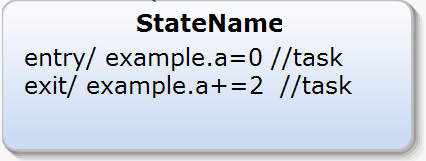
\includegraphics[width=60mm, keepaspectratio]{figures/state.png}
\caption{\label{fig:state}Egy állapot Yakinduban.}
\end{figure}

A rendszer természetesen működés közben változik, másik állapotba kerül. Az állapotváltást a tranzíciók segítségével írjuk le. Ezeket mindig valamilyen esemény váltja ki, lehet egy felhasználói esemény, vagy egy időzített esemény. Őrfeltételt is adhatunk \verb+[]+-en belül ilyenkor csak akkor lépünk át a másik állapotba, ha ez a feltétel teljesül. A \verb+/+ után pedig újabb parancsokat hajthatunk végre

\begin{figure} [!ht]
 	\centering
 	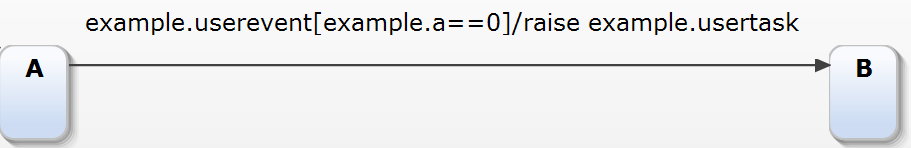
\includegraphics[width=150mm, keepaspectratio]{figures/transition.png}
 	\caption{\label{fig:transition}Egy tranzíció Yakinduban.}
\end{figure}

Előfordulhat az is, hogy több állapotot valamilyen közös tulajdonságuk szerint szeretnénk csoportosítani. Ilyenkor jók az összetett állapotok.\label{infovesztes} Ezt az információt veszítjük tehát el, ha "kilapítjuk"\footnote{Több állapot felvételével helyettesítjük az összetett állapotokat} az állapotgépet.

Itt kell bevezetni a régió fogalmát. Minden állapot egy régióban van, és minden régióban egyszerre csak egy állapot írhatja le a rendszerünket. Az összetett állapotok tehát tartalmaznak legalább egy régiót.

A régión belül van egy úgynevezett pszeudó állapot, ami kijelöli, hogy egy régióba lépés esetén melyik állapotba lépjünk. Három fajtája van a history, deephistory és a sima kezdő állapot. A sima mindig ugyanarra az állapotra mutat, a history megjegyzi, hogy kilépéskor melyik volt aktív és oda léptet vissza. A deephistory még ennél is többet jegyez meg, ha a kilépéskori aktív állapot, egy összetett állapot, akkor az azon belüli aktív állapotokat is megjegyzi.

\begin{figure} [!ht]
	\centering
	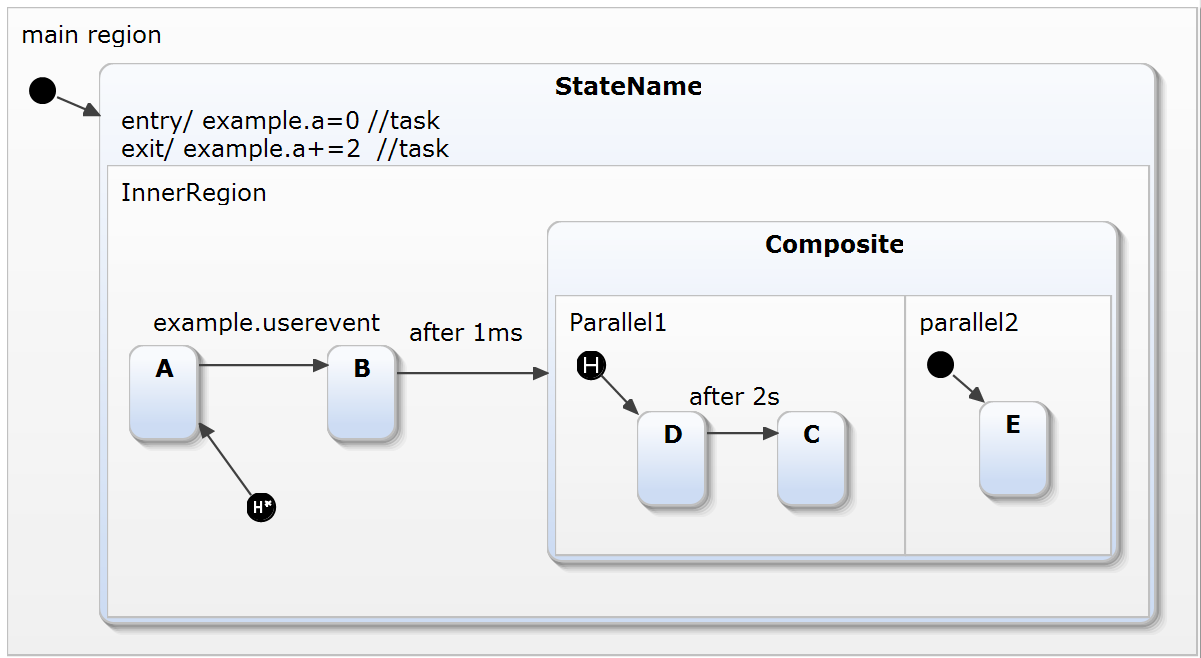
\includegraphics[width=150mm, keepaspectratio]{figures/statechart.png}
	\caption{\label{fig:statechart}Egy összetett állapotgép Yakinduban.}
\end{figure}


%----------------------------------------------------------------------------
\section{A {\thetaSc}}
\label{sec:thetaleiras}
%----------------------------------------------------------------------------

Az állapotgép reprezentáció Java-ban készült el. Az egyes osztályok megfeleltethetők az előző fejezetben leírt állapotgép elemekkel. Mindegyik osztálynak vannak a tárolt elemeihez getter/setter, a tárolóikhoz pedig add függvényei. Illetve néhány segédfüggvény, ami segít majd az analízis közben. A projekt már korábbi munkák folytatásaként jött létre. Az én hozzájárulásom a pszeudó állapotok implementálása, az időzített események kezelése és néhány segéd függvény, illetve apróbb javítások.


\begin{lstlisting}[language=java,breaklines=true]
interface Sc {}
\end{lstlisting}

Az állapotgépet reprezentáló interfész. Ez tárolja a gyökér régiót. Van neve, tárolja az összes tranzíciót az állapotgépben. Tárolja a változó deklarációkat egy a Thetában értelmezett osztályban (VarDecl). 

Az egyetlen megvalósító osztály a \verb+MutableSc+ minden tárolója hashSet-ben van megvalósítva

\begin{lstlisting}[language=java,breaklines=true]
interface Region {}
\end{lstlisting}

Van neve, tárolja az állapotait (State), ezek lekérdezhetőek és pontosan egy pszeudó állapota (PseudoState) van. Lehet szülő állapota; az állapot ami közvetlen őt tartalmazza. Továbbá van egy Boolean attribútuma, ami azt jelzi, hogy RootRegion-e a régió azaz nincs neki szülőállapota. Ellenőrizhető, hogy szabályos-e a régió: Minden tartalmazás igaz fordított irányban (vagyis az elem szülő eleme a régió)

Az egyetlen megvalósító osztály a \verb+MutableRegion+ egy hashSet-ben tárolja az állapotait

\begin{lstlisting}[language=java,breaklines=true]
interface State {}
\end{lstlisting}

Van neve és tárolja a régióit (Region) ez lehet egy üres lista. Kötelezően van szülő régiója. Van két akciója (Action), egy a kimeneti, egy a bemeneti akcióknak. Van két tranzíció tárolója, tárolja ugyanis a beérkező tranzíciókat és a kimenőket is.

Az egyetlen megvalósító osztály a \verb+MutableState+ minden tárolója hashSet-ben van megvalósítva

\begin{lstlisting}[language=java,breaklines=true]
interface Transition {}
\end{lstlisting}

A tranzíciót reprezentáló interfész. Tárolja a forrás állapotát (honnan indul ki) és a cél állapotát (hova érkezünk). Továbbá van egy kiváltó (trigger) eseménye (Event). Lehet őrfeltétele, ami a Thetában is használt Expr<Type> osztály. Van egy akciója (Action)

Az egyetlen megvalósító osztály a \verb+MutableTransition+

\begin{lstlisting}[language=java,breaklines=true]
interface PseudoState {}
\end{lstlisting}

Van neve, tárolja azt az egy állapotot ami a régiójába lépéskor az aktuális állapot lesz. Kötelezően kell legyen egy szülő régiója (Region).

Három megvalósító osztály a \verb+MutableInitState+ a sima kezdő ~ a \verb+MutableHistorytate+ a history~ a \verb+MutableDeepHistoryState+ pedig a deephistory pszeudó állapothoz

\begin{lstlisting}[language=java,breaklines=true]
interface Action {}
\end{lstlisting}

Interfész az akcióknak. Visitor mintát követi. Négy különböző osztály van. 

Az \verb+AssignmentAction+ egy egyszerű változó értékadást reprezentál, van tehát egy változója (VarDecl) és egy kifejezése (Expr).

A \verb+SignalAction+ egy esemény (Event) jelzést reprezentál. Ennek megfelelően tárol egy eseményt (csak egyet)

Az \verb+EmptyAction+ azért van, hogy ne null-okat tároljunk ha egy tranzíciónak, vagy állapotnak nincs akciója

A \verb+SequenceAction+ Több akciót (Action) tárol

\begin{lstlisting}[language=java,breaklines=true]
interface Event {}
\end{lstlisting}

Az eseményeket reprezentáló interfész alapvetően, csak egy neve van.

Két megvalósító osztály van az \verb+EventImpl+ a user eseményekhez, a \verb+TimeEventImpl+ pedig az időzített eseményeknek a \hyperref[fig:statechart]{3.3-as ábrán} is látható after 2s is egy ilyen esemény. Tárolja a nevén kívül azt, hogy mennyi az időzítés (milliszekundumban).


%----------------------------------------------------------------------------
\section{Sorosítás}
%----------------------------------------------------------------------------

Amikor egy adott modellen akarunk végezni analízist, valószínűleg nem csak egyszer tesszük ezt meg, hanem többször is. Nem lenne túl hatékony, ha mindig újra kéne építeni az állapotgépet, erre van a sorosítás, vagy szerializáció, ami lehetővé teszi az állapotgépek gyors beolvasását, illetve akár néhány módosítás utáni kiírását.

A séma Lisp-szerű szintaxist követ. A \hyperref[sec:thetaleiras]{fent} említett elemek sorosítva a következőképp néznek ki:

\begin{lstlisting}[language=java,breaklines=true]
(statechart nameOfStateChart
	(var varName varType)
	(var var2 type)
	(event Esemény)
	(region regionName
		(state stateName
			(entry assign varName value)
			(exit assign var2 value))
		(state compositeState
			(region innerRegion
				(state inState)
				(state stateA))
				(init inState))
		(history stateName))
	(transition stateName compositeState
		(trigger Esemény)
		(guard varName>2)
		(effect 
			(sequence
					(assign varName value)
					(signal Esemény))))
\end{lstlisting}

Azt érdemes megemlíteni, hogy egy-egy elemet előbb deklarálunk, például (var varName varType) és utána már elég a nevével hivatkozni rá. Például (assign varName value)

\begin{figure} [!ht]
	\centering
	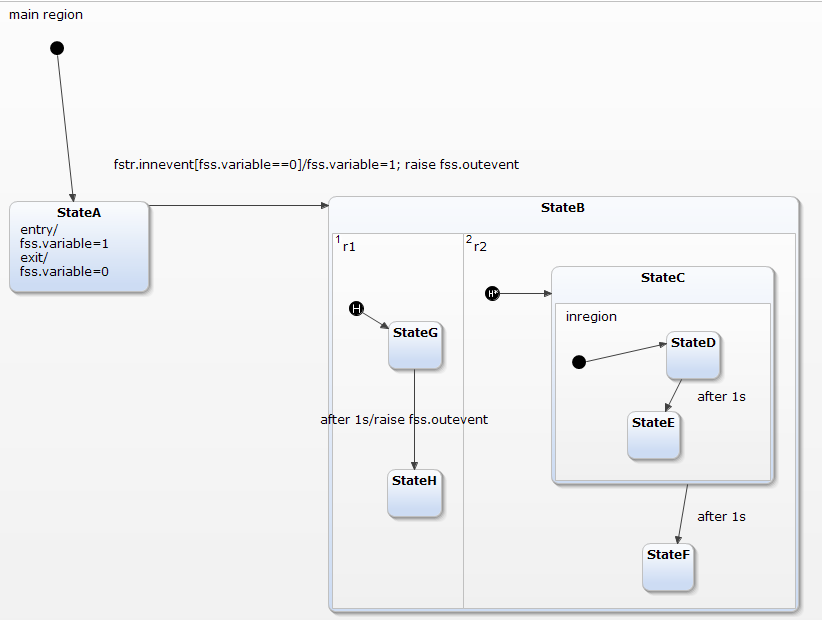
\includegraphics[width=150mm, keepaspectratio]{figures/serializeexample.png}
	\caption{\label{fig:serializeexample}példa állapotgép a szerializációhoz}
\end{figure}

\begin{figure} [!ht]
\centering
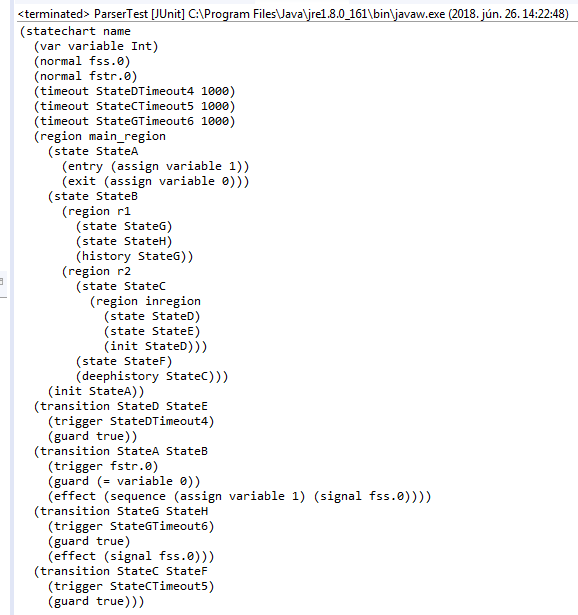
\includegraphics[width=150mm, keepaspectratio]{figures/serializeresult.png}
\caption{\label{fig:serializeresult}a \hyperref[fig:serializeexample]{fenti} állapotgép sorosítva}
\end{figure}


%%----------------------------------------------------------------------------
\chapter{\transzformacio}
\label{sec:transzformacio}

A Gamma keretrendszert is szeretnénk összekötni az \hyperref[sec:thetaleiras]{előző} fejezetben bemutatott {\thetaSc}pel. Ezért írtam egy segéd osztályt, ami képes a beolvasott EMF-es {\gammaSc}et átalakítani {\thetaSc}pé.
%----------------------------------------------------------------------------
\section{{\gammaSc}}
%----------------------------------------------------------------------------
Már korábban említettem az \hyperref[sec:archiutecture]{Architektúra} fejezetben, hogy a {\gammaSc} egy EMF alapú állapotgép reprezentáció. Így a sémája nem sokban különbözik az \hyperref[sec:thetaleiras]{előző} fejezetben leírt {\thetaSc}től. Ez megkönnyíti a transzformáció folyamatát. Az erre a célra írt segédosztályokat mutatom be a következő részekben


%----------------------------------------------------------------------------
\section{GammaSctoThetaSCConverter}
%----------------------------------------------------------------------------

Ez az osztály egy statikus \verb+convert()+ függvény meghívásával transzformál

\begin{lstlisting}[language=java ,breaklines=true]
public static MutableSc Convert(final StatechartDefinition gammaSC, final String name) 
\end{lstlisting}

Látható, hogy bemenetként egy beolvasott EMF gyökér elemet várunk (ez a {\gammaSc}et reprezentáló StatechartDefinition osztály) a name pedig a {\thetaSc} neve lesz.

Először beolvassuk a változókat, ezekkel létrehozok egy ExpressionConverter-t amit a következő szekcióban mutatok be. Utána beolvassuk a gyökér régiót ami az addRegiontoThetaSC() rekurzív függvény meghívásával történik utána a tranzíciókat adom az állapotgéphez (frissítve a már korábban létrehozott állapotokat)

\begin{lstlisting}[language=java ,breaklines=true]
private static void addRegiontoThetaSC(final Region reg, final MutableRegion r) 
\end{lstlisting}

Ez a függvény rekurzív, abból a szempontból, hogy ha egy régión belül van egy másik régió akkor meghívja önmagát. Minden elemhez van egy ehhez hasonló függvény, aminek a bemenete, egy gammás elem és egy annak megfelelő Thetás elem, és a transzformátor a gammás elemben lévő belső elemeket létrehozza és berakja a Thetás elembe. Ez így megy addig amíg az adott elemekben vannak újabb elemek.

%----------------------------------------------------------------------------
\section{ExpressionConverter}
%----------------------------------------------------------------------------

A legnagyobb nehézség az akciókban illetve őrfeltételekben használt kifejezések megfelelő átkonvertálása, ehhez használom a ExpressionConverter segéd osztályt. A Thetában van erre egy segítség a DispachTable. Ennek a segítségével könnyen és átláthatóan össze lehet kötni a különböző gammás Expression-öket a Thetás Expr<> osztályokkal

%%----------------------------------------------------------------------------
\chapter{Állapotgép konfiguráció}
\label{sec:stateconfig}
%----------------------------------------------------------------------------
\section{Aktív állapot}
%----------------------------------------------------------------------------
Az állapotgép a rendszerünk összes lehetséges állapotát mutatja. Analízis közben azonban fontos hogy azt is tudjuk nézni, hogy mik az aktív állapotok, azaz melyek írják le a rendszerünk pillanatnyi helyzetét.

Az aktív állapotoknak van több szabálya.
\begin{itemize}
	\item Egy régión belül, pontosan egy aktív állapot lehet (közvetlen gyerekekre nézve)
	\item Egy aktív állapot összes szülő állapota is aktív
	\item Minden régióban van aktív állapot
\end{itemize}

%----------------------------------------------------------------------------
\section{A megvalósító osztály}
%----------------------------------------------------------------------------

A StateConfiguration osztályban valósítom meg. Egy ilyen példány tartalmazza az állapotgép reprezentációt (Sc) továbbá egy listát az épp aktuális állapotokról és -egy később igen hasznosnak bizonyuló segítség- tároljuk, hogy az adott konfiguráció mely tranzíciók elsütésével érhető el a kiindulási állapotból, illetve hogy eközben milyen akciók lettek végrehajtva. Oly módon, hogy minden egyes tranzícióhoz ebben a listában két akció tartozik, egy azokhoz az akciókhoz, amik a tranzíció őrfeltétel ellenőrzés előtt hajtódnak végre, egy pedig azokhoz amik utána.

\begin{lstlisting}[language=bash,morekeywords={sudo,apt\-get},alsoletter={-},breaklines=true]
public static StateConfiguration create(final Sc sc)
\end{lstlisting}

Létrehozható egy {\thetaSc}ből.

\begin{lstlisting}[language=bash,morekeywords={sudo,apt\-get},alsoletter={-},breaklines=true]
public void init()
\end{lstlisting}

Aktiválja az állapotgépet, azaz mindenhol a kezdő állapot szerint kijelöli az aktív állapotokat

\begin{lstlisting}[language=bash,morekeywords={sudo,apt\-get},alsoletter={-},breaklines=true]
	public Collection<Transition> getFireableTransitions()
\end{lstlisting}

Visszaad egy listát az összes olyan tranzícióról, ami tüzelhető az adott konfigurációban. Vagyis a tranzíció forrásállapota aktív.

\begin{lstlisting}[language=bash,morekeywords={sudo,apt\-get},alsoletter={-},breaklines=true]
public StateConfiguration fire(final Transition tr)
\end{lstlisting}

Visszaad egy új állapotgép konfigurációt, ami a paraméterben megadott tranzíció elsütése után kialakul. Saját magát nem változtatja!


%%----------------------------------------------------------------------------
\chapter{Korlátos modell ellenőrző}
\label{sec:bmc}
%----------------------------------------------------------------------------
\section{Modell ellenőrzés}
%----------------------------------------------------------------------------
A \hyperref[sec:intro]{bevezetőben} már elmondtam miért fontos a modellellenőrzés, most inkább arról beszélek, hogy ez mit jelent az állapotgépek esetén. A \hyperref[fig:mcheck]{6. 1-es ábrán} látható a működés elve. A modellellenőrző tehát egy modell reprezentációt, és egy tulajdonságot kap bemenetként. És megadja, hogy teljesül-e az adott tulajdonság, vagy nem. Ilyenkor még egy példát is ad arra, amikor nem teljesül, amivel könnyen ellenőrizhetjük, hogy igaz volt-e. A másik esetben viszont, ha nem talál ellenpéldát akkor azt bebizonyítani, hogy valóban nincs, csak úgy lehet, ha a modellellenőrző működés közben bizonyítottan megtalál minden ellenpéldát. Ezt sokszor csak bizonyos korlátok mellett lehet biztosítani.

A tulajdonság, általában egy elérhetőségi vizsgálatot jelent\footnote{Elérhető-e egy állapot a kezdeti állapotkonfigurációból, úgy, hogy minden tranzíció elsütése érvényes, azaz teljesül az őrfeltétel}. A BMC\footnote{Bounded Model Checker, a korlátos modell ellenőrző rövid neve}-nél sincs ez másképp, ilyenkor az ellenpélda egy útvonal az elérni kívánt állapothoz\footnote{Mely tranzíciókat kell elsütni, milyen sorrendben}. Mivel azt szeretjük, ha a hibás esetekben van ellenpélda ez az állapot egy hibaállapot, ami a rendszer nem megfelelő működését jelzi.

A BMC a helyes működést, azaz hogy egy állapot biztosan nem érhető el nem tudja bizonyítani, mert végtelen ideig is tarthatna a futás ideje. Ezért inkább megfogalmaz egy korlátot: maximum K lépésből elérhető-e az adott állapot

\begin{figure}[!ht]
	\centering
	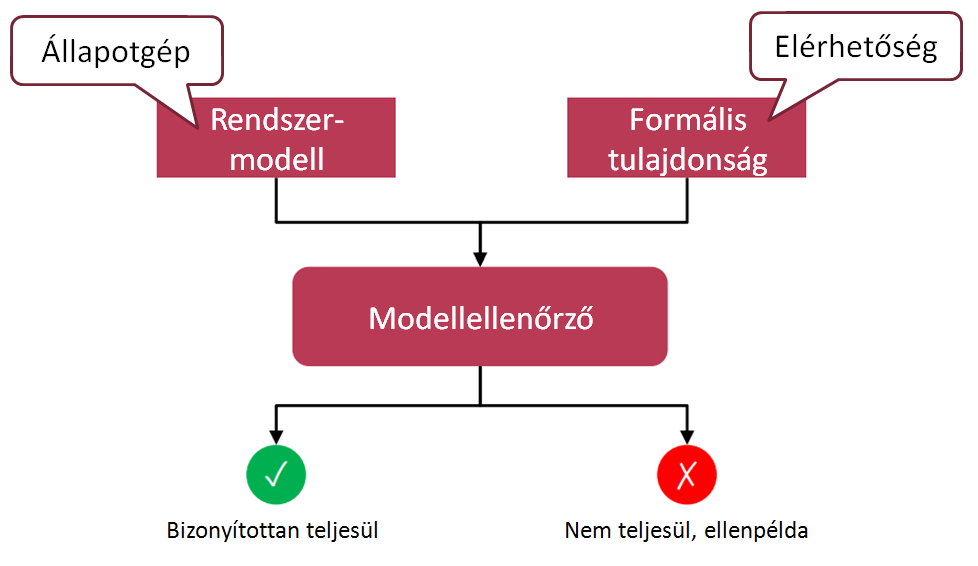
\includegraphics[width=74mm, keepaspectratio]{figures/altmc.png}\hspace{0cm}
	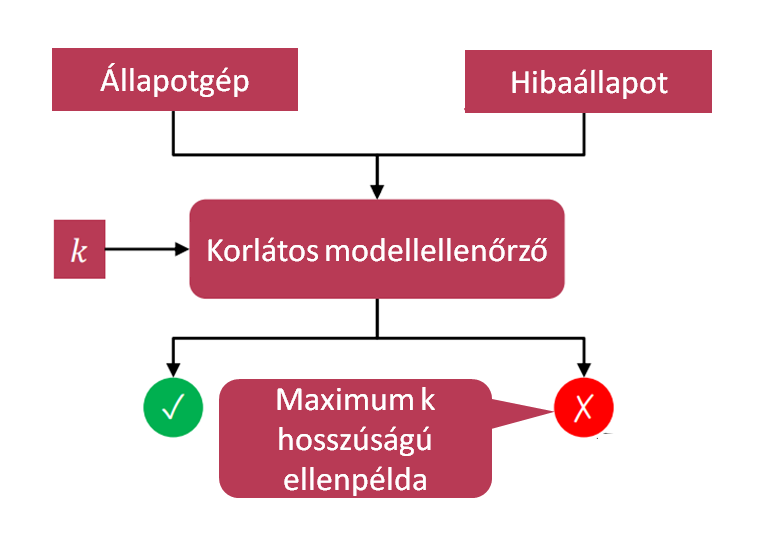
\includegraphics[width=74mm, keepaspectratio]{figures/bmc.png}
	\caption{Az általános ~ (balra) és a korlátos modellellenőrző (jobbra) működési elve}
	\label{fig:mcheck}
\end{figure}


%----------------------------------------------------------------------------
\section{A BMC menete}
%----------------------------------------------------------------------------
A korlátos modellellenőrző működése a \hyperref[fig:bmcfolyamat]{6.2-es ábrán} látható. A keresés egy szélességi gráf
bejárás az állapotkonfigurációkon ahol a k korlát mélységig megyünk. A hiba állapot olyan állapotgép konfigurációt jelent, ahol a hibaállapot aktív.

\begin{figure}[!ht]
	\centering
	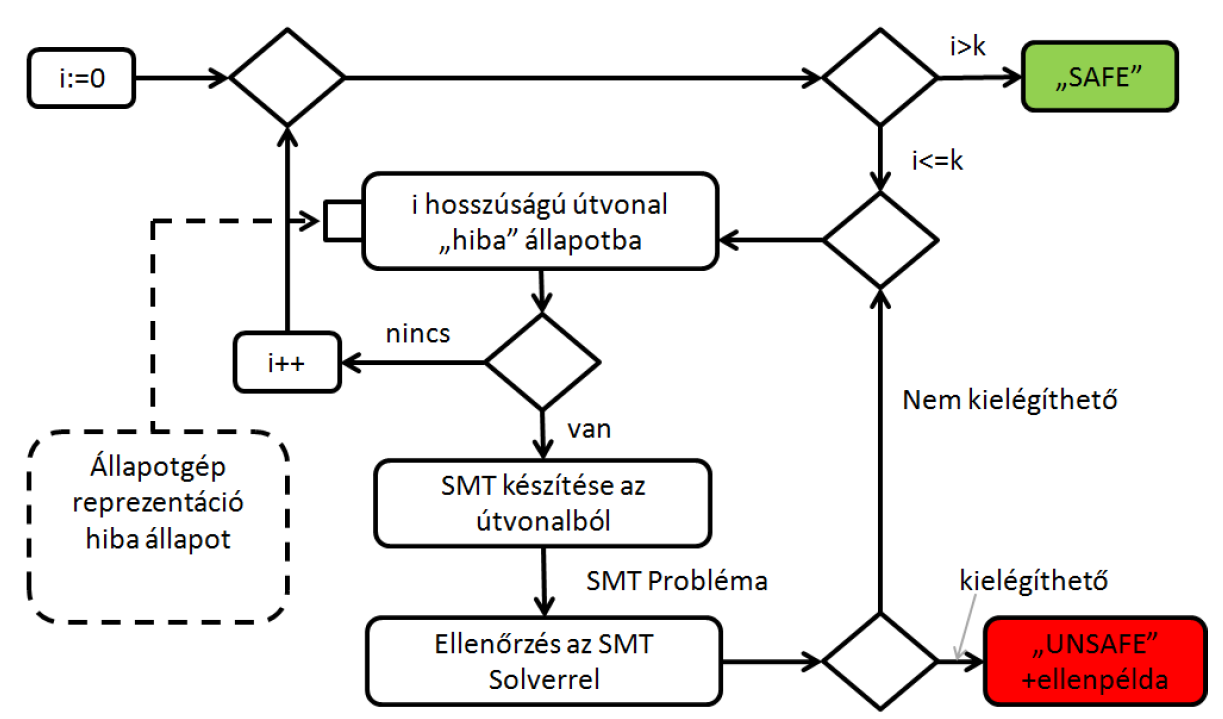
\includegraphics[width=150mm, keepaspectratio]{figures/bmcfolyamatmodell.png}
	\caption{A korlátos modellellenőrző folyamat modellje}
	\label{fig:bmcfolyamat}
\end{figure}

%----------------------------------------------------------------------------
\section{Az útvonal}
%----------------------------------------------------------------------------
A \verb+Path+ osztályt használom ennek a leírására. Tárolom az összes állapotgép konfigurációt az kiinduló állástól kezdve, és az útvonal során elsütött tranzíciókat.


\begin{lstlisting}[language=java,breaklines=true]
public boolean checkpath()
\end{lstlisting}

Azt ellenőrzi, hogy az útvonal helyes-e azaz minden egyes konfigurációból valóban jó konfigurációba léptünk és az elsütött tranzíció elsüthető volt (a forrásállapota aktív volt)

\begin{lstlisting}[language=java,breaklines=true]
public StateConfiguration getResultConfiguration()
\end{lstlisting}

Az útvonal végigfutása utáni állapotkonfigurációt adja vissza


%----------------------------------------------------------------------------
\section{SMT Solver}
%----------------------------------------------------------------------------
Az SMT solver egy olyan eszköz, ami több aritmetikai kifejezést kapva, megtudja mondani, hogy ezek teljesülhetnek-e egyszerre. Ha igen akkor ad egy példa értéket az összes benne szereplő változóra, hogy azok kielégítsék mindegyik aritmetikai kifejezést.

Ezek most nekünk azért kellenek, mert az útvonalakon, a tranzíciókon lévő őrfeltételek is egy ilyen aritmetikai kifejezéshalmazt képeznek. 

A Theta projektben van egy interfész a Z3 solveréhez, ezt használtam.

Az \verb+SMTBuilder+ segéd osztályban csinálok az útvonalak segítségével SMT problémát, amit át tudok adni a solvernek.

\begin{lstlisting}[language=java,breaklines=true]
public SMTBuilder(final Path p) {
\end{lstlisting}
A segéd osztály egyszerűen létrehozható az útvonal alapján.


\begin{lstlisting}[language=java,breaklines=true]
public Collection<Expr<BoolType>> unfold()
\end{lstlisting}

Ezzel a függvénnyel hozzuk létre azt a listát, amit közvetlen átadhatunk a solvernek. 

Elsőre egyszerűnek tűnik, hiszen a tranzíciók, már ezt a formátumot használják az őrfeltételek tárolásához, de figyelemmel kell kísérni azt is, hogy az akciók során változhatnak a változó értékei -akár többször is-. Ennek a problémának a megoldásához van egy eszköz a Theta projekten belül (\verb+PathUtils+), ami pont ennek a "változó frissítésnek" ad implementációt. Itt válik hasznossá, hogy az \hyperref[sec:stateconfig]{állapotgép konfigurációkban tároljuk az összes akciót, ami a kezdeti állapothoz képest történt}.

%----------------------------------------------------------------------------
\section{BoundedChecker}
%----------------------------------------------------------------------------
Maga az ellenőrző osztály a \verb+BoundedChecker+.

\begin{lstlisting}[language=java,breaklines=true]
public BoundedChecker(final Sc chart, final int K, final State errorState)
\end{lstlisting}

Bemenetként egy állapotgépet várunk, amin végezzük az ellenőrzést. Bekérünk egy K korlátot, ami megadja a maximum lépés számot, és persze maga a hiba állapotot is kell.

\begin{lstlisting}[language=java,breaklines=true]
	public SafetyStatus check()
\end{lstlisting}

Ezzel a függvénnyel lehet futtatni az ellenőrzést, egy \verb+SafetyStatus+ al tér vissza amiből kiolvasható, hogy biztonságos-e, ha nem, akkor az ellenpéldát is ki lehet olvasni. Meghívja az \verb+algorithm+ függvényt

\begin{lstlisting}[language=java,breaklines=true]
public SafetyStatus algorithm(final Collection<Path> paths, final int deep) 
\end{lstlisting}

Egy rekurzív függvény ami, minden egyes lépésben növeli a mélységet (deep) és, minden útvonalból, (ami nem bukott már meg) létrehozza az összes lehetséges új útvonalakat. Ehhez elég az útvonal utolsó konfigurációján minden elsüthető tranzíciót elsütni.

Így biztosítjuk azt, hogy az összes lehetséges útvonalat megnézzük, aminek a hossza az inicializáláskor megadott maximumnál nem nagyobb. Tehát, ha nem találunk ellenpéldát akkor biztosan állíthatjuk, hogy nincs is.

A bizonyítás azért nem ennyire egyszerű, mert ugyan kipróbálunk minden lehetőséget, előfordulhat, hogy egy jó ellenpéldát nem fogadunk el, ez persze úgy lehet, ha például, rosszul építjük meg az SMT problémát és azt kapjuk, jogtalanul, hogy az útvonal nem teljesíthető.

További információ a \hyperref[sec:verifikacio]{verifikációs} résznél



%%----------------------------------------------------------------------------
\chapter{Verification}
\label{sec:verifikacio}

%----------------------------------------------------------------------------
\section{The Abstraction library usage}
%----------------------------------------------------------------------------
Implementing an abstraction type:

Run reachability analysis:

%----------------------------------------------------------------------------
\section{Performance measurements}
%----------------------------------------------------------------------------


%----------------------------------------------------------------------------
\section{Tests on the implemented abstraction algorithms}
%----------------------------------------------------------------------------



%\include{content/latex-tools}
%\include{content/thesis-format}
%\include{content/template-usage}


% Acknowledgements
%~~~~~~~~~~~~~~~~~~~~~~~~~~~~~~~~~~~~~~~~~~~~~~~~~~~~~~~~~~~~~~~~~~~~~~~~~~~~~~~~~~~~~~
%\include{content/acknowledgement}


% List of Figures, Tables
%~~~~~~~~~~~~~~~~~~~~~~~~~~~~~~~~~~~~~~~~~~~~~~~~~~~~~~~~~~~~~~~~~~~~~~~~~~~~~~~~~~~~~~
%\listoffigures\addcontentsline{toc}{chapter}{\listfigurename}
%\listoftables\addcontentsline{toc}{chapter}{\listtablename}


% Bibliography
%~~~~~~~~~~~~~~~~~~~~~~~~~~~~~~~~~~~~~~~~~~~~~~~~~~~~~~~~~~~~~~~~~~~~~~~~~~~~~~~~~~~~~~
%\addcontentsline{toc}{chapter}{\bibname}
%\bibliography{bib/mybib}
\chapter*{\referencia}\addcontentsline{toc}{chapter}{\referencia}
\label{sec:ref}

[1] \hyperref[src:http://web.mit.edu/16.399/www/lecture_01-intro/Cousot_MIT_2005_Course_01_4-1.pdf]{Patrick Cousot: An informal overview of abstract interpretation}

[2] Cousot, P. and R. Cousot, Abstract interpretation: A unified lattice model for static analysis of programs
by construction of approximations of fixed points

[3] Eric Goubaulta, St´ephane Le Rouxb, Jeremy Lecontec, Leo Libertib, and Fabrizio Marinellid: Static Analysis by Abstract Interpretation: A Mathematical Programming Approach

[4] \hyperref[src:https://inf.mit.bme.hu/en/theta]{Theta framework}

% Appendix
%~~~~~~~~~~~~~~~~~~~~~~~~~~~~~~~~~~~~~~~~~~~~~~~~~~~~~~~~~~~~~~~~~~~~~~~~~~~~~~~~~~~~~~
%\include{content/appendices}

%\label{page:last}
\end{document}
